% Intended LaTeX compiler: pdflatex
\documentclass[runningheads,a4paper]{llncs}
\usepackage[utf8]{inputenc}
\usepackage[T1]{fontenc}
\usepackage{graphicx}
\usepackage{grffile}
\usepackage{longtable}
\usepackage{wrapfig}
\usepackage{rotating}
\usepackage[normalem]{ulem}
\usepackage{amsmath}
\usepackage{textcomp}
\usepackage{amssymb}
\usepackage{capt-of}
\usepackage{hyperref}
\institute{}
\titlerunning{REVIEW 1337777.OOO SOLUTION PROGRAMME}
\author{}
\date{}
\title{REVIEW 1337777.OOO SOLUTION PROGRAMME : 1337777 MOM PENTAGON IS SOME RECURSIVE SQUARE}
\hypersetup{
 pdfauthor={},
 pdftitle={REVIEW 1337777.OOO SOLUTION PROGRAMME : 1337777 MOM PENTAGON IS SOME RECURSIVE SQUARE},
 pdfkeywords={},
 pdfsubject={},
 pdfcreator={Emacs 25.1.2 (Org mode 9.0.3)}, 
 pdflang={English}}
\begin{document}

\maketitle
\begin{abstract}
The 1337777.OOO SOLUTION PROGRAMME originates from some
random-moment dia-para-computalogical discovery of some convergence of
the DOSEN PROGRAMME \url{http://www.mi.sanu.ac.rs/\~kosta} along the COQ
PROGRAMME \url{https://coq.inria.fr}.  This memo presents that some
random-moment new angle of view, that 1337777 mom associativity
pentagon is some recursive square (reflective-functorial
bracket-elimination cut-elimination resolution), onto some decades-old
associativity-coherence question may solve some common falsification
in mathematics. Moreover the computational-logical content of this new
angle of view is programmed into the COQ computer
\url{https://gitlab.com/1337777/maclane/blob/master/maclaneSolution2.v} . En
passant, this memo confirms that the only real mathematical research
or industry is the predictable-time (1337) « engineering » of some
computational-logical software with varying degree of
logical-constraints, and everything else is the education or teaching
of random-moment (777) dia-para-computalogical « ideas ».  This
grammatical bracket-elimination cut-elimination resolution technique
is the saint holy halo oxygene of all the computer programming of
polymorph mathematics by the 1337777.OOO SOLUTION PROGRAMME.
Necessarily, the 1337777.OOO has discovered
random-moment dia-para-computalogic ,
forced-fool-and-theft / lie / falsification ( « absence of reality »
). Necessarily, the 1337777.OOO has discovered
information-technology to measure
reviews/citations (¢entse currency) by using public programmatic
proxy-authors « pprogxy » ( « ethereum blockchain smart-contract » )
integrated along content-addressable personal-public
replicated-storage ( « swarm dht » ).
\keywords{1337777.OOO ; COQ ; associativity coherence ; Maclane ; angle of view ; bracket-elimination ; cut-elimination ; confluence ; coherence ; polymorph functors ; metafunctors-grammar ; duality}
\end{abstract}

\section{Outline}
\label{sec:org7ef4c06}

This memo presents some new lemma, that 1337777 mom associativity
pentagon is some recursive square (reflective-functorial
bracket-elimination cut-elimination resolution), which is held in the
real deduction of the associativity coherence, because Maclane's old
deduction-attempt is not the reality. Moreover the
computational-logical content of this random-moment new angle of view
is programmed into the COQ computer 
. This lemma constructs some adjunction functor from the associativity
category of words-objects and bracketing-arrows to (the opposite of)
the semiassociativity (oriented bracketing-arrows) category. Elsewhere
this associativity coherence is the meta-terminology for the
completeness-lemma of another semiassociativity coherence , and this other semiassociativity coherence
does lack some more-common Newman-style local confluence lemma.

One corresponding phrasing to describe any adjunction functor is to
start by giving the unit of the adjunction (here the normalization of
words) and then by giving the universality-map of this unit of the
adjunction. This new angle of view is that this recursive square is
precisely one such given half of this universality-map, but it is
sufficient.  As shown in this view :

\begin{figure}\centering 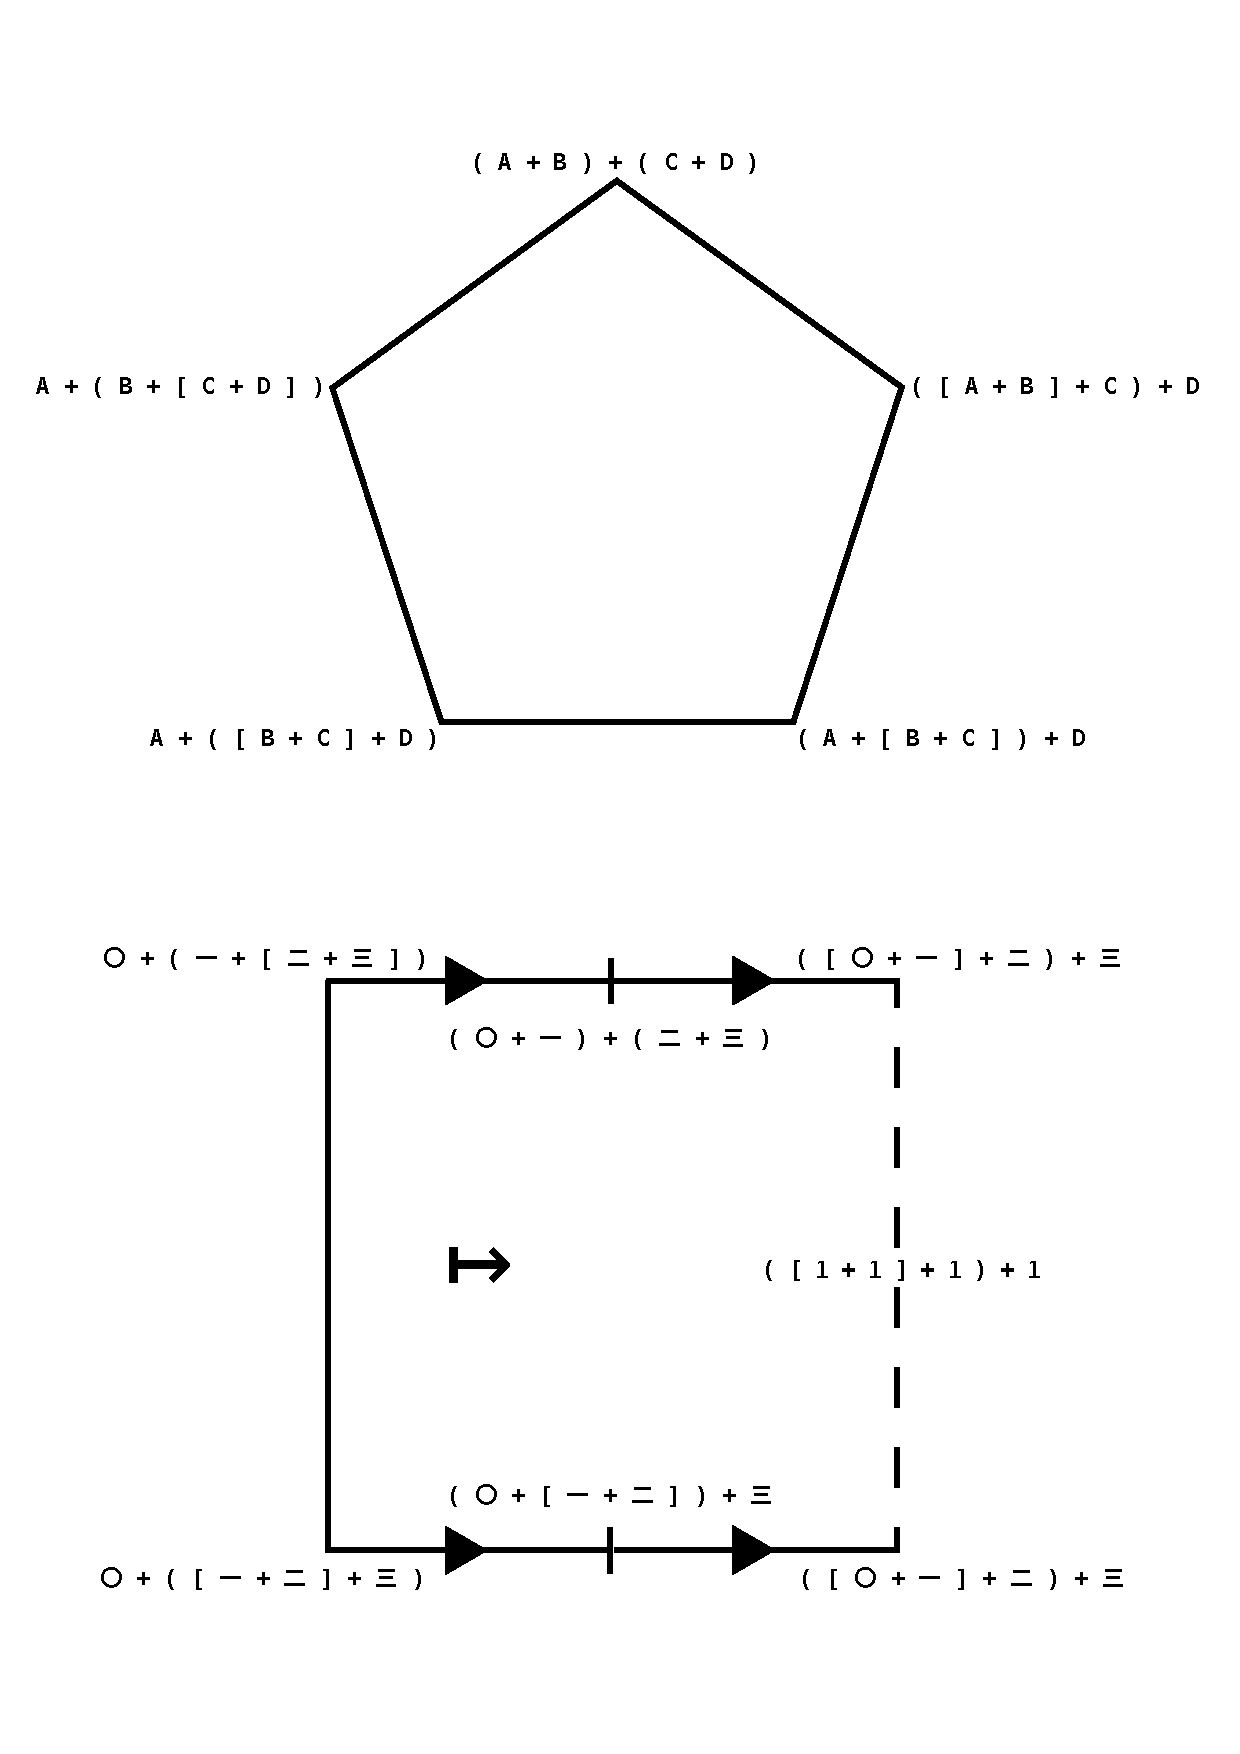
\includegraphics[scale=0.5]{maclaneSolution.svg.pdf} \caption{View}\end{figure}
\end{document}
